\subsection{Análise de Ruído das operações}

Nesta seção estão as análises do crescimento de ruído das operações entre criptogramas RLWE e RGSW.
\subsubsection*{Soma Homomórfica $C_1 \boxplus  C_2$}
O ruído dessa operação pode ser calculado por:
$$
Err(C_1 \boxplus  C_2) = sk^T(C_1 + C_2) - (\mu_1 + \mu_2)sk^TG
$$
Organizando,
$$
Err(C_1 \boxplus  C_2) = sk^T(C_1) - (\mu_1)sk^TG + sk^T(C_2) - (\mu_2)sk^TG = e_1^T + e_2^T 
$$

\subsubsection{Multiplicação Homomórfica $C_1 \boxdot C_2$}
O ruído desta operação pode ser calculado por
$$
Err(C_1 \boxdot C_2) = sk^\top(C_1G ^{-1}(C_2)) - (\mu_1\mu_2)sk^\top \mathbf{G}
$$
Expandindo a expressão encontra-se:
$$
Err(C_1 \boxdot C_2) = (1,-s) \begin{pmatrix} s \mathbf{a}_1^\top + \mathbf{e}_1^\top \\ \mathbf{a}_ 1^\top \end{pmatrix}G ^{-1}(C_2) + \mu_1(1,-s)\begin{pmatrix} s \mathbf{a}_2^\top + \mathbf{e}_2^\top \\ \mathbf{a}_ 2^\top \end{pmatrix}
$$
Simplificando, finalmente:
$$
Err(C_1 \boxdot C_2) = \mathbf{e}_1^\top G ^{-1}(C_2) + \mu_1 \mathbf{e}_2^\top
$$

O produto externo padrão entre RGSW e RLWE pode ser calculado por

$$C_1 \boxtimes c_2 = \begin{pmatrix} s \mathbf{a}_1^\top + \mathbf{e}_1^\top \\ \mathbf{a}_ 1^\top \end{pmatrix}g^{-1}(c_2) + \mu_1\mathbf{G}g^{-1}(c_2)$$ 
$$=\begin{pmatrix} s \mathbf{a}_1^\top g^{-1}(c_2) + \mathbf{e}_1^\top g^{-1}(c_2) \\ \mathbf{a}_ 1^\top g^{-1}(c_2) \end{pmatrix} + \begin{pmatrix} s a_2 \mu_1 + \mu_1 \mu_2 \frac{Q}{B} + \mu_1 e_2 \\ a_2 \mu_1 \end{pmatrix} $$
$$=\begin{pmatrix} s ( \mathbf{a}_1^\top g^{-1}(c_2) + a_2\mu_1) + \mu_1\mu_2\frac{Q}{B} +  \mathbf{e}_1^\top g^{-1}(c_2) +\mu_1 e_2 \\ \mathbf{a}_ 1^\top g^{-1}(c_2) + a_2 \mu_1 \end{pmatrix}$$
Finalmente, o ruído é calculado por:
$$
Err(C_1 \boxtimes c_2) = \mathbf{e}_1^\top g^{-1}(c_2) +\mu_1 e_2  
$$
Dessa forma, a sua norma infinita deve ser
$$
||Err(C_1 \boxtimes c_2)||_\infty < 2\ell N||e_1||_\infty + \mu_1 ||e_2||_\infty 
$$

\subsubsection{Subgaussiana}
Para a análise de ruído 'justa' é preciso utilizar que parte das variáveis aleatórias trabalhadas são limitadas por distribuições 
subgaussianas. A intuição é de que podemos encontrar um limite superior probabilístico utilizando a desigualdade de Markov se soubermos
a distribuição que rege a variável aleatória. 

\begin{definition}
    Para \( s > 0 \), define-se a função Gaussiana \( \rho_s : H \to (0,1] \) por
\[
\rho_s(\mathbf{x}) = \exp\left(-\pi \|\mathbf{x}\|_2^2 / s^2\right).
\]
A distribuição Gaussiana contínua \( D_s \) é obtida pela normalização de \( \rho_s \), com densidade \( s^{-n} \cdot \rho_s(\mathbf{x}) \).

Define-se também que uma variável aleatória \( X \in \mathbb{R} \) é \( \delta \)-subgaussiana com parâmetro \( s > 0 \) se, para todo \( t \in \mathbb{R} \),
\[
\mathbb{E}[\exp(2\pi t X)] \leq \exp(\delta + \pi s^2 t^2).
\]

\end{definition}

Agora tome as seguintes propriedades presentes em \cite{lyubashevsky2013} e \cite{lw23I}.

\begin{lemma}[Lema 3.2 \cite{lw23I}]
    \textit{Para quaisquer cifras RGSW} $\mathbf{C}_1, \mathbf{C}_2$ \textit{que cifram} $\mu_1, \mu_2$ \textit{com termos de erro} $\mathbf{e}_1, \mathbf{e}_2$ \textit{respectivamente, temos o seguinte:}

    \[
    \text{Err}(\mathbf{C}_1 \boxplus \mathbf{C}_2) = \mathbf{e}_1^\top + \mathbf{e}_2^\top.
    \]

    \[
    \text{Err}(\mathbf{C}_1 \boxtimes \mathbf{C}_2) = \mathbf{e}_1^\top \cdot \mathbf{G}^{-1}(\mathbf{C}_2) + \mu_1 \cdot \mathbf{e}_2^\top.
    \]

    \textit{Além disso, suponha que} $\mathbf{G}^{-1}$ \textit{é amostrado com respeito a alguma base} $\mathbb{Z}$ \textit{de} $\mathcal{R}$, \textit{isto é,} $\mathbf{B} = \{ \mathbf{b}_1, \dots, \mathbf{b}_n \}$, \textit{tal que} $\max_{i \in [n]} \{ \| \sigma(\mathbf{b}_i) \|_\infty \} \leq 1$ \textit{como no Lema 2.3. Então os seguintes fatos valem:}

    \begin{itemize}
    \item Denote $\mathbf{e}_1^\top \cdot \mathbf{G}^{-1}(\mathbf{C}_2)$ como $\mathbf{e}^\top = (e_1, \dots, e_{2\ell})$. Então cada entrada de $\mathbf{e}$ é uma variável aleatória independente.

    \item $\|\sigma(\mathbf{e})\|_\infty$ é limitada superiormente por uma variável sub-Gaussiana com parâmetro $O(r)$, para algum $r > 0$ tal que $r \leq \sqrt{N \cdot \log Q} \cdot \|\sigma(\mathbf{e}_1)\|_\infty$.
    \end{itemize}
\end{lemma}

\begin{lemma}
    Seja uma variável aleatória $X$ de distribuição gaussiana de parâmetros $(\mu = 0, \sigma)$, esta variável é limitada superiormente
    por um subgaussiana de parâmetro mínimo $\sqrt{2\pi}\sigma$
\end{lemma}

Com o último lema, garantimos que a amostragem gaussiana do erro reflete em uma variável subgaussiana. Logo, passamos para uma análise dos ruídos acumulados pelo resto das operações.

\subsubsection{Key Switch}
O algoritmo de key-switch, tem como função a troca de chave de um criptograma cifrado
em uma chave antiga $s'$, para uma chave nova $s$, o que aumenta o ruído gerado na cifra, vamos verificar quanto.
Para que o algortimo seja realizado corretamente, é necessário 
que seja passado como parâmetro a \textit{lower half} de um criptograma $RGSW_s(s')$, ou seja, é necessário assumir 
que o RGSW tem segurança circular.

Seja então $d \in \text{RLWE}_{s'}(\mu)$ e $d = (a, b)$, e queremos então um criptograma de $\mu$ cifrado em $\text{RLWE}_{s}$.
Considere então $K$ a \textit{lower half} de um criptograma $RGSW_s(s')$. O objetivo então é encontrar o ruído gerado por, 
$$
[0,b] - K \times g^{-1}(a)
$$
Como $K$ é a parte inferior de $RGSW_s(s')$ considere $K = (A, As + gs' + \mathbf{e}_{KS}) \in \mathcal{R}_Q^{2 \times \ell}$. Desenvolvendo,

$$
-(g^{-1}(a) \times A), -(g^{-1}(a) \times A) s + \mu \frac{Q}{B} + E - \mathbf{e}_{KS} g^{-1}(a)
$$
Note que o vetor obtido é um criptograma valido $\in \text{RLWE}_{s}(\mu)$ com ruído 
$E - \mathbf{e}_{KS} g^{-1}(a)$ que possui norma infinita correspondente:
$$
||Err(KS(d))||_\infty < ||Err(d)||_\infty + N\ell ||\mathbf{e}_{KS}||_\infty
$$
No teorema 4.6 de \cite{lw23I}, assume-se que $Err(d)$ e $\mathbf{e}_{KS} g^{-1}(a)$ são subgaussianas com um mesmo parametro $B$, o que é coerente visto que a magnitude do ruído do key-switch deve ser muito menor do que a da mensagem $d$. O key switch foi implementado em SageMath e C++.

\subsubsection{Eval-Trace}

Para facilitar a análise de ruído do algoritmo 4.1 de \cite{lw23I}, considere o mesmo
algoritmo simplificado, para o efeito da acumulação do ruído ser mais visível, a variável $d$ terá um 
índice que representa seu degrau na torre de extensão. 

\begin{algorithm}[H]
\caption{(RLWE)-Eval-Tr\(_{K/K_{13}}\) com a estrutura de torre}
\SetKwInOut{Input}{Entrada}
\SetKwInOut{Output}{Saída}

\Input{
\begin{itemize}
  \item \(c = (b, a) \in (\mathcal{R}_1 \otimes \mathcal{R}_2 \otimes \mathcal{R}_3)^2\) que encripta uma mensagem \(\mu \in \mathcal{R}_1 \otimes \mathcal{R}_2 \otimes \mathcal{R}_3\) sob um segredo \(s \in \mathcal{R}\).
  \item \(\{\text{evk}^{(\sigma)}\}_{\sigma \in \bigcup_{i=1}^{t-1} \text{Gal}(E_i/E_{i+1})}\), e \(\text{evk} \in \text{RGSW}_s(P^{-1} \cdot s) \in \mathcal{R}^2\).
\end{itemize}
}
\Output{
\(c_{out} \in \text{RLWE}_s(\text{Tr}_{K/K_{13}}(\mu))\).
}

Inicialize \(c = (b, a)\), defina \(\bar{a} = P \cdot a\) \\
Calcule \(d_0 = \text{evk} \boxtimes (0, \bar{a})\) \\
\For{\(i = 1\) até \(t - 1\)}{
  Calcule \(d_{i+1} = \sum_{\sigma \in \text{Gal}(E_i/E_{i+1})} \text{KS}( \sigma(d_i), \text{evk}^{(\sigma^{-1})})\)\\
}
Retorne \((\text{Tr}_{K/K_{13}}(b), 0) - d_n\) 

\end{algorithm}
Assuma sem perda de generalidade que o traço realizado é $K \rightarrow K_{13}$.
Começaremos analisando a recurssão do loop na linha 4:
$$
d_{i+1} = \sum_{\sigma \in \text{Gal}(E_i/E_{i+1})} \text{KS}( \sigma(d_i), \text{evk}^{(\sigma^{-1})})
$$
Então, utilizando a expressão do erro do key-switch:
$$
Err(d_{i+1}) = \sum_{\sigma \in \text{Gal}(E_i/E_{i+1})} Err(\sigma(d_i)) - e_{KS}^{\sigma} g^{-1}(d_i[0])
$$
Perceba que $Err(\sigma(d_i)) = \sigma(Err(d_i))$ e que o segundo termo no somatório tem sua norma limitada por um valor pequeno,
em uma análise inicial $N\ell ||e_{KS}^{\sigma}||$, utilizando o lema 3.2 é uma variável subgaussiana com parâmetro limitado por 
$\sqrt{N\ell} ||e_{KS}^{\sigma}||$. Visto que sua norma independe do seu estágio na torre, troque-o por $e'$ onde $||e'|| \le  N\ell ||e_{KS}^{\sigma}||$. Logo, 
$$
Err(d_{i+1}) < p_2 e'+ \sum_{\sigma \in \text{Gal}(E_i/E_{i+1})} \sigma(Err(d_i))
$$
Observe que o termo $\sum_{\sigma \in \text{Gal}(E_i/E_{i+1})} \sigma(Err(d_i)) = Tr_{E_i / E_{i+1}}(Err(d_i))$ 
$$
Err(d_{i+1}) < p_2 e' + Tr_{E_i/E_{i+1}}(Err(d_i))
$$
A partir dessa recorrência, é possível chegar na relação:
$$
Err(d_{n}) < Tr_{K / K_{13}}(Err(d_0)) + \rho' e'
$$
Sabendo que $d_0 = evk \boxtimes [0, \bar{a}]$, $Err(d_0) = Err(evk) g^{-1}([0, \bar{a}])$.
Tome $f$ como o criptograma resultante, $f = (\text{Tr}_{K/K_{13}}(b), 0) - d_n$. Então, expressão  do ruído toma a forma:
$$
Err(f) < Tr_{K / K_{13}}(e) + Tr_{K /K_{13}}(Err(d_0)) + \rho' e'
$$
Ao considerar que as normas de ruído de $\mathbf{e}_{KS}$ e $evk$ são limitadas pelo mesmo valor $E$, temos que $||Tr_{K /K_{13}}(Err(d_0))|| < 2N \ell E$, logo
aplicando as normas:
$$
||Err(f)|| < ||Tr_{K /K_{13}}(e)|| +  3 \rho'N\ell E
$$

Lembrando que $||e||$ é a norma do ruído do criptograma inicial. Note que no teorema 4.6 de \cite{lw23I} é proposta uma análise mais justa do erro, a única 
diferença é que os produtos da forma $\mathbf{e} g^{-1}(x)$, onde $||\mathbf{e}|| < E$ são subgaussianos com parametros limitados. Tal operação foi implementada em SageMath e C++.

\subsubsection{\emph{framework} Ext-Prod}
Tome $\delta_i^{(j)}$ como a componente $i$ do ruído da mensagem $\mu_i^{(j)}$ empacotada cifrada em RGSW e  $e_i^{(j)}$ como a componente $i$ do ruído da mensagem $d_j$ resultante empacotada em RLWE. 

Analisado o resultado após Com o resultado da seção anterior e com o erro do produto externo, temos:
$$
e^{(1)} < Tr_{K / K_{13}}(\sum_i \delta_i^{(1)} v_i^v w_i g^{-1}(d_0) + \mu^{(0)} e_i^{(0)}v_i) +  \Delta
$$
Onde $||\Delta|| < 3 \rho'N\ell E$. Se aplicarmos a norma infinita da expressão, conseguimos obter:
$$
||e^{(1)}|| < \frac{2\rho (p_2-1)N\ell}{\rho'}\sum ||\delta_i^{(1)}|| + \rho ||\mu^{(1)}||\sum||e_i^{(0)}|| + 3 \rho'N\ell
$$
Perceba que essa expressão é análoga a expressão obtida no artigo ao efetuarmos uma análise utilizando variáveis subgaussianas.

\subsubsection{$k$ Aplicações}
Calcular o ruído após $k$, com $k$ par, operações onde as mensagens são $\mu_i^{(j)} = \xi_q^{t^{(j)}_i}$ simulando o que ocorre durante o batch bootstraping. Substituindo a expressão [], pelas variáveis definidas:
$$
e^{(k)} < \sum_i e_i^{(k-1)} \xi_q^{t^{(k)}_i} w_i + Tr_{K / K_{13}}(\sum_i \delta_i^{(k)} v_i^v w_i g^{-1}(d_{k-1})) +  \Delta
$$
Vamos replicar a mesma coisa para $k-1$ lembrando que agora o traço efetuado será relativo ao corpo $K_{12}$:
$$
e^{(k-1)} < \sum_i e_i^{(k-2)} \xi_q^{t^{(k-1)}_i} v_i + Tr_{K / K_{12}}(\sum_i \delta_i^{(k)} w_i^v v_i g^{-1}(d_{k-2})) + \Delta'
$$
onde $||\Delta'|| \le 3 \tau'N\ell E$. Agora temos que isolar as componentes de $e^{(k-1)}$ utilizando o traço, por definição do dual temos:
$$
e_i^{(k-1)} = Tr_{K /K_{13}} (e^{(k-1)} v_i^v)
$$
Desenvolvendo este sistema, encontramos o resultado que:
$$
||e^{(k)}|| < ||e^{(0)}||+ \frac{k}{2}(4 p_2p_3r^2 + 6 p_2r \tau' + 2r p_2 + 3 \rho' ) N (\log Q) E
$$
Sobre a análise 'justa', utilizando o lema 8.3, basicamente o que mudam são as normas das operações envolvendo os vetores $g$, artigo ajustasse o parâmetro da subgaussiana para $r \sqrt{N \log Q} E$ tendo assim como resultado final:  
$$
||e^{(k)}|| < ||e^{(0)}||+ \frac{k}{2}(4 p_2p_3r^2 + 6 p_2r \tau' + 2r p_2 + 3 \rho' ) r \sqrt{N \log Q} E
$$
Note que esta operação foi implementada em SageMath e C++. Observe as figuras a seguir comparando o crescimento da norma infinita do ruído:

\begin{figure}[H]
  \centering
  \begin{subfigure}{0.45\textwidth}
    \centering
    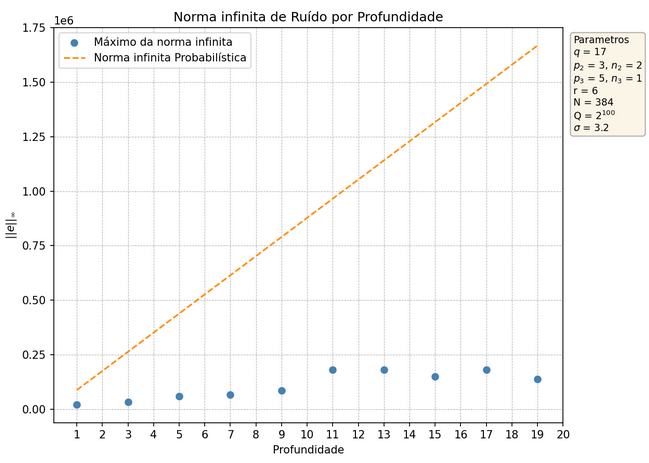
\includegraphics[width=\linewidth]{sections/images/image2.png}
  \end{subfigure}
  \hfill
  \begin{subfigure}{0.45\textwidth}
    \centering
    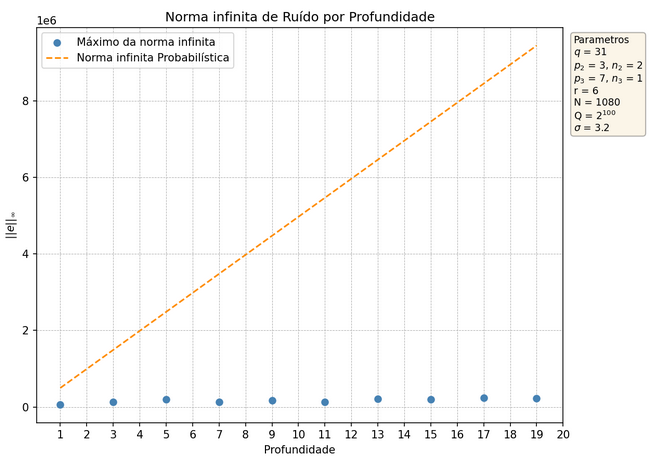
\includegraphics[width=\linewidth]{sections/images/image.png}
  \end{subfigure}
  \caption{Gráficos da norma infinita pela quantidade de produtos externos realizados }
\end{figure}

Para a geração destes \emph{plots} foram omitidas as constantes dos primos, levou-se em conta apenas as variáveis relacionadas ao parâmetro de segurança, $O(r^3\sqrt{N\log Q}E)$. Perceba que mesmo assim, existe uma distância bem razoável entre o ruído encontrado e o limite probabilistíco encontrado. Dado estes e outros testes, é um bom indicativo que escolher os parâmetros da forma utilizada pelo artigo, com a constante da análise assintótica sendo $1$ é, de fato, condizente com a realidade.

